\documentclass[0-thesis.tex]{subfiles}

\begin{document}
With the required background information, an architecture for an update mechanism can be
proposed. Five key areas that the architecture must deal with have been identified:

\begin{itemize}
    \item Roles
    \item Key distribution and management
    \item Authorization and access control
    \item Means of communication
    \item Upgrading images
\end{itemize}

The architecture must propose solutions for these four areas while complying with SUIT as
much as possible in order to make the architecture interoperable and suitable as a
standard. Certain elements, such as how to locally flip an image and which kinds of
authorization tokens to issue, are implementation dependant. The architecture must however
support different means of achieving these goals and not restrict engineers to one certain
implementation.

Alongside these four key areas is the concern of a devices life cycle from an update
perspective. The life cycle should be intertwined with the mechanisms of the architecture
and show how devices can enroll, communicate, and receive updates throughout their long
expected lifetimes. 

Section~\ref{sec:roles} defines what a server and operator means in the context of the
update mechanism. Section~\ref{sec:key-management} discusses what is needed for devices to
enroll in a PKI and how keys are handled during updates. Section~\ref{sec:authorization}
describes the purpose of issuing authorization tokens, how devices can use them, and who
is to be authorized. Section~\ref{sec:communication} describes how devices, servers, and
operators can communicate and shows an example workflow of communicating an update.
Section~\ref{sec:updates} discusses different means of handling the payload when applying
an update. Section~\ref{sec:device-lifecycle} introduces the notion of a life cycle for
devices, and Section~\ref{ssec:different-architectures} shows different examples of
possible architectures.

\section{Roles}
\label{sec:roles}
This Section~explains the notion of servers and operators in the architecture and their
responsibilities. Section~\ref{ssec:who-is-a-server} covers the topic of servers while
Section~\ref{ssec:who-is-an-operator} covers operators.

\subsection{Who Is a Server and What Do They Do?}
\label{ssec:who-is-a-server}
% Server: dedicated server or other device in network. Identified by keys, needs to be on
% devices? Single point of truth for device profiles and versions. Can be used as storage
% for images being deployed later on.
% TODO: Mention pre-determined lists of servers
Servers are responsible for transporting manifests and images to the devices and keeping
track of device profiles. Upon enrollment devices register at a server and the server
creates a profile for that device. The profile contains the vendor and class IDs and
firmware version of the device. This allows the server to know through which protocols the
device can be contacted and which version it should be updated to. Operators, discussed in
the next section, send signed manifests and images to servers, and can query them for
device status.

Devices should contain a list of servers and by trusting the certificate authority, they
can validate those machines certificates after being enrolled. A server is thus any
machine that is enrolled, has a valid certificate, and is included in the devices list of
servers. The reasoning behind this decision is that a standard solution for updates should
not assume the topology of an IoT network. The server may be a machine acting as a proxy
between a traditional network containing the operator and a constrained network with IoT
devices. The server could be a more capable IoT device located entirely within the
constrained network and be contacted through a proxy. The server could be located entirely
within the traditional network and use a proxy to communicate with devices of the
constrained network.

% TODO: Does a device need one keypair for each server? Does it need one keypair for all servers?
A device could also be aware of several servers, and different devices can be mapped to
different servers. This can make device management easier as certain classes of devices
can be handled by certain servers. By allowing a device to receive updates from several
servers, the update mechanism architecture displays a form of robustness. If one server is
a machine located entirely within the constrained network and the connection between that
server and the operator is severed, updates can still be distributed through other
servers. If devices are pulling updates, they can query the servers in order of their list
of servers. If updates are pushed, devices keep the connection with the server pushing the
update.

Which machines are allowed to act like servers can be boiled down to a few important
points no matter the topology of choice:

\begin{itemize}
    \item The server is enrolled and has a valid certificate
    \item The server is included in a devices list of servers (meaning it is authorized to
            transport updates to the device)
    \item An operator can reach the server and is authorized by the server to upload
            updates
\end{itemize}

What servers are allowed to do must also be predetermined. Imagine a device running an
operating system and an application. The operating system is developed by some party
different than the one developing the application, and thus the device is aware of two
update servers, one for the operating system and one for the application. If receiving an
update from the application update server, the device should allow for the update to
happen but also make sure the correct parts of code are updated. The application vendor
should not be allowed to touch the operating system if they are not authorized to do so,
and vice versa. This introduces the topic of authorizing updates. Authorization and access
control is discussed in Section~\ref{sec:authorization}.

\subsection{Who Is an Operator and What Do They Do?}
\label{ssec:who-is-an-operator}
% Operator: human making decisions about updates. Crafts/generates manifests, signs
% manifests and images. Authorized by keys, needs to be on device? Can send manifest for
% ease of operations, cannot send images because of size constraints/single point of
% truth/proxying? How does an operator send manifests, get profile from server? Must get
% profiles anyways for versioning.
% TODO: Mention pre-determined list of operators. Mention it can be updated just like any
% other piece of software
Operators are people authorized to upload manifests and images to a server. They can also
optionally upload manifests directly to a device depending on the architecture. Operators
prepare manifests and images and signs them before transporting them to a server, which
forwards them to a device. The signing ensures end-to-end security for images and
manifests between operators and devices.

Like a list of servers introduced in Section~\ref{ssec:who-is-a-server}, devices also need
a list of operators. This is because if an operator wishes to send a manifest directly to
a device, the device needs to know if the operator is authorized to do so, otherwise it is
discarded. Just like with mapping devices to servers, devices can receive manifests from
several operators and different devices may interact with different operators. This
creates opportunities to logically divide a network between different operators. An
example use case is a constrained network supported by different vendors; the respective
vendors should only be able to service their respective devices despite all devices
belonging to the same network. It can also create a hierarchy, where certain operators may
directly interact with devices but other operators must interact with devices through
servers. Yet again the point is to prepare for as many different scenarios as possible and
create a flexible architecture.

As with servers, the essence of being an operator can be captured in a few points:

\begin{itemize}
    \item An operator is enrolled and has a valid certificate
    \item An operator is included in a devices list of operators (and therefore can send
            manifests to the device)
    \item An operator is trusted by a server to send manifests and images to the server,
            causing devices to update
\end{itemize}

Access control for operators is an important topic. Operators should only be able to send
updates to devices they are authorized for, and the updates should cover parts of the
device within the operators rights. Section~\ref{sec:authorization} discusses access
control for operators and servers.

% TODO: Briefly explain what is ment by "device"

\section{Key Management}
\label{sec:key-management}
% TODO: Consider updates breaking certificates. Why would they? Lack of understanding concerning
% certificates perhaps
% Two pairs of keys from one PSK? Are two pairs needed?
The architecture will, in order to align with the goals of SUIT, be based on asymmetric
cryptography. The availability of EST-coaps makes this feasible in IoT contexts but other
enrollment protocols could also be used. This means a \gls{ca} is needed to act as a
trusted third party distributing certificates. The certificates are linked to a public key
which has a private key partner and are used to verify the correctness of a public key.
Certificates are signed by the CA and in order to trust them, device have to trust the CA
itself.

In order to enroll, a pre-shared key is proposed. This is the approach used in EST-coaps,
but it is not chosen for that reason. If a pre-shared key is not used the CA cannot be
sure the device asking to enroll really should be part of the trusted network. An attacker
that obtained a valid certificate could communicate with devices and servers alike and no
one would be able to tell it is a malicious actor. CAs must know they are issuing
certificates to the correct devices and pre-shared gives devices a means of identifying
themselves. Pre-shared keys could be used for encrypting all traffic but as they are less
scalable and harder to manage than certificates, they are just used for enrolling.

A device that is enrolling has to trust the CA issuing the certificate. If it cannot do
so, how could it know it received a valid certificate? An attacker would love for a device
to use the attackers public key instead, and if an attacker poses as a CA it could issue a
certificate with its own public key and then sign it. In order to trust the CA, a device
needs to have the certificate of the CA it is enrolling with or some other CA further down
the chain of trust. By verifying the signature on the newly enrolled certificate with the
CAs own certificate, a device can be certain they are using the correct keys.

When applying updates, certificates might not be valid anymore. This is implementation
dependant and might not always be a problem, but the architecture should be prepared for
these situations. In the case an update breaks a certificate, the certificate cannot be
used for communication and thus the device cannot use it to re-enroll either. In this
case, a new pre-shared key should be part of the update so that the device can enroll as
if it was factory new. The process of issuing pre-shared keys might be difficult to
automate as the CA must be aware of which keys to accept, but it is needed to ensure the
security of future device communication.

\section{Authorization}
\label{sec:authorization}
% TODO: Maybe put this after communication?
A flexible architecture enables different configurations of servers, operators, and
devices. An operator might be authorized to update all parts of all devices, or be
constrained to updating a specific piece of functionality for a subset of the devices.
Operating system vendors might be allowed to push security updates for the operating
system but not change the application code. Controlling access rights is a security issue
and the architecture must support it.

How clients can access a protected resource through authorization tokens is described in
\parencite{ace} and Figure \ref{fig:ace-flow} shows an adaptation of the protocol flow
from that document. The figure shows how a client wanting to access a resource requests a
token from an authorization server. The token is returned to the client, which can then
send a request and token to the server holding the resource. If necessary, the resource
server can send an introspection request to the authorization server asking for more
information about the token in order to verify it. If everything goes as planned, the
client is allowed the resource.

In the context of the update architecture, the client would be a party needing to
authorize themselves, i.e. an operator or server. The access token would have to be of a
lightweight variant since they are to be used on constrained devices, but which variant is
implementation specific. Tokens will be sent with updates (signed manifests and images) to
devices, the resource sought for is the ability to update the device. The device will thus
not respond with a particular resource, but instead if the token is valid recognize the
originator of the update as an authorized one and proceed with the update. Introspection
is an interesting feature of ACE since it requires less from the device concerning
validating tokens. Instead of doing everything on its own, the device can ask the server
for additional information making the validation procedure easier. This however means some
extra communication which is power consuming for an IoT device. To use introspection or
not is yet again an implementation issue, but authorization servers should be both
enrolled and reachable for devices to send introspection requests if necessary.

\begin{figure}
    \caption{The protocol flow of ACE. Adapted from \parencite{ace}.}
    \label{fig:ace-flow}
    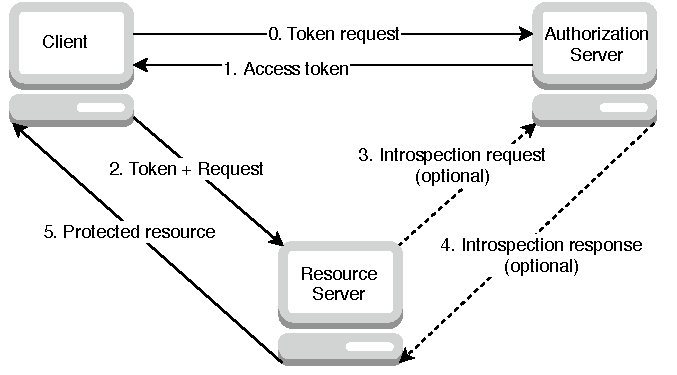
\includegraphics{images/ace.pdf}
\end{figure}

Who is supposed to authorize? As updates will be sent from operators through servers to
devices, the devices need to know the originator of an update is authorized to issue the
update. The proposition is to only require operators to authorize. No matter how updates
are initiated or distributed (pull vs push and manifest and image together vs separately),
updates at some point must be crafted, signed, and sent by an operator. The operator is
making the decisions about updating, and thus must authorize these decisions through
tokens. Servers deliver the updates to devices, but do so as a relay for operators, as
well as acting as repositories for images and device profiles. The messages forwarded by
servers will contain the authorization token granted to an operator. This token can in
addition to authorizing the update on a device be used by the server to authorize the
usage of the server by the operator. 

Not requiring servers to authorize should not pose any issues as the update must be
prepared in a previous step by an operator that authorizes. Also, it makes the flow of
applying an update easier by not needing communication to the authorization server by an
update server. Requiring update servers to authorize would not add any security to the
devices as the update already will be shipped with a token authorizing the update.

\section{Communication}
\label{sec:communication}
In heterogeneous networks of IoT devices, each device might sport a specific protocol
stack. In order to enable different devices to be updated, servers must be aware of how to
reach these devices. This problem introduces the notion of device profiles containing
information about device capabilities and software versions. 

When devices have enrolled and obtained a valid certificate, they must contact their
respective servers so the servers can create profiles of the devices. The profiles will
tell through which protocols to reach a device and what software versions the device is
using. In order to achieve this, devices must first know which servers to contact. This
can be solved through shipping devices with a list of servers. This list can later on be
updated like any other software. Furthermore, the devices use vendor and class IDs as
described in the SUIT information model. The information model uses these pieces of
information to verify an update is intended for a specific device by matching the IDs, but
they can also be sent to a server to tell it what kind of device is contacting it. The
server can infer a profile based on the IDs it is sent, or simply use the protocols the
device chose to contact it. The devices also need to be aware of how to register, for
instance by POSTing to a specific server endpoint. 

When updating there are possibilities regarding how the updating process is initiated. An
operator can query the server for the status of one or several devices, prepare an update
for them, and have the update pushed through the server. Optionally the operator could
send a manifest to the device explaining when the update is to be applied and put the
image on the server. Later when the device should update, the device pulls the image from
the server, validates it using the already received manifest, and updates. Both the pull
and push approaches assume the devices are already enrolled and registered at the server.

\begin{figure}
    \caption{Example workflow of an update procedure.}
    \label{fig:communication-workflow}
    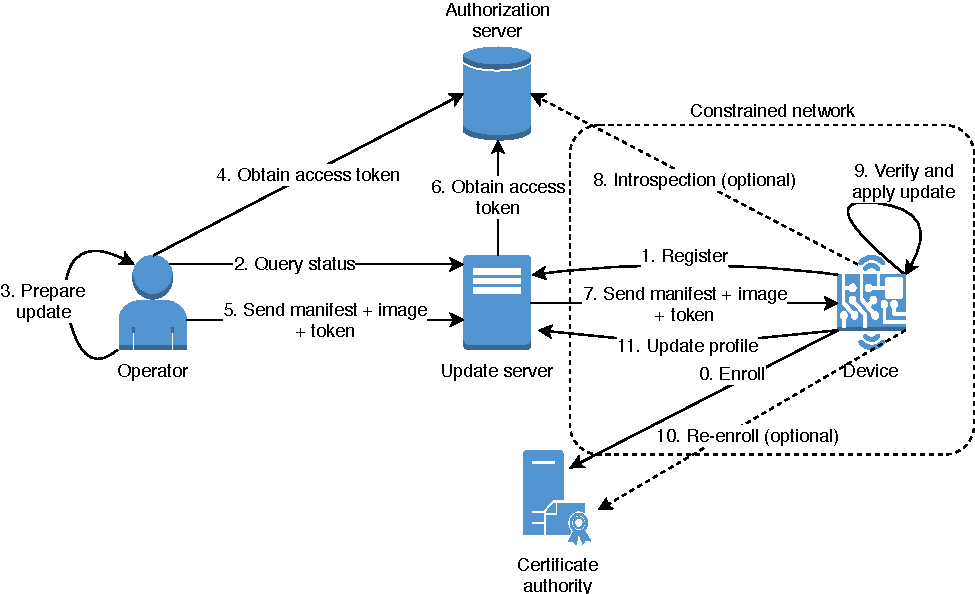
\includegraphics{images/update-flow.pdf}
\end{figure}

Figure~\ref{fig:communication-workflow} shows an example update flow in the architecture.
This update is initiated by the operator by querying the server for device status and then
pushing an update. The manifest and image are distributed together.

\begin{enumerate}[label=0.\arabic*]
    \setcounter{enumi}{-1}
    \item Enrolling the device at the certificate authority.
    \item Registering at the server. This creates a profile for the device on the server.
    \item The operator prepares a manifest and signs it.
    \item The operator requests an access token from the authorization server in order to
            gain access to applying the update.
    \item The manifest and image are both signed and sent to the server with the
            authorization token.
    \item The signed manifest and image are sent with the authorization token to the
            device.
    \item The device optionally requests introspection data from the authorization server
            to verify the authorization token.
    \item The device confirms the update if successful and causes the server to update
            its device profile.
\end{enumerate}

After updating, the devices capabilities might have changed, for instance by having a new
protocol implemented in software. The version has also changed due to applying an update.
After an update, a device should notify all its servers so they can update the device
profile (or simply discard the old one and generate a new, as if the device registered for
the first time). This ensures the servers view of the devices is up to date and that
communication will always happen through the intended and supported protocols. The
functionality of registering is the same as when a device is new and thus not costly to
implement.

There are alternatives to using device profiles. One alternative is to instead keep a list
of known protocols implemented by devices in the network, and when pushing updates to a
device trying each protocol in sequence. This has the benefit of not needing to keep and
continuously update profiles, but also has some issues. One issue is that you still need
to keep some state of the devices on the server regarding firmware version. If the server
does not know what the status of device versions are, it cannot help a human operator
decide about deploying updates. 

Another drawback is that devices might implement common protocols but have different
preferences. If two devices implement some common protocols but one of them supports
hardware operations for encrypting one of the protocols, it will prefer using that
protocol with the server, whereas the other device might not. The server will however,
with no information about device preference, try the same sequence of protocols with both
devices.

Furthermore, as communication can be unreliable over these networks, the server
cannot know for sure if a device does not respond due to not understanding the protocol
and therefore dropping the packets, or if the response just got lost in transmission. It
is more robust to keep track of which protocols devices support and conform to the
preferences of the constrained devices.

Lastly, instead of using profiles all communication could be initiated from the device
side, meaning updates are only done through a pulling mechanism. This would not enable the
use case of pushing updates which could be critical if a vulnerability must be patched
right away. Operators must be given the choice to push updates to their devices, and thus
servers must be able to initiate contact with devices.


\section{Updates}
\label{sec:updates}
% TODO: How to handle decryption and validation
% I like the idea of decrypting once and storing decrypted image with its hash for smaller
% bootloader procedure. Implementation specific though
% Cite mailing list perhaps?

When an update has finally arrived to the device, it must be processed and then installed.
The process of decrypting, validating, and installing the image is heavily implementation
specific with most of the details being out of scope for the architecture. However, since
devices operate using different hardware and bootloaders they must be given the freedom
to update in the way that makes most sense for them. The architecture should support this.

By delivering optional fields such as decryption instructions, processing steps, and
postconditions, update handlers and bootloaders can take care of updates in various ways.
This enables different ways of applying updates within the same architecture. What the
update handlers and bootloaders of all devices have in common is that they must trust the
source of the update, they must be able to decrypt the update, they must be able to verify
the validity of the update, and they must be able to do this safely such that an
unexpected power cycle does not brick the entire device.

Still being in the realm of very constrained devices, the bootloader should be as simple
as possible. This is also a requirement stated by SUIT on the architecture. By decrypting
and verifying the image at every boot the boot procedure will be secure but
quite complex. Also if a power cycle occurs during decryption, the device might not be
able to recover. Decrypting the image as part of the update mechanism and writing it
unencrypted to flash would allow for a simpler bootloader, but is less secure as the
device would boot from an unencrypted image.

By storing the manifest containing the image digest, unencrypted images can be verified by
comparing their digest to the one in the manifest. Digests are easier to calculate than
decryption is, and a power cycle would just interrupt the digest calculation instead of
the decryption of the actual bootable image. In order to make sure the manifest is correct
upon boot, the digest of the manifest can be calculated and stored alongside the manifest
and image. The manifest also has to be stored in order to prevent rollback attacks. It
contains monotonically increasing sequence numbers to ensure devices do not install older,
possibly vulnerable images, but in order to compare sequence numbers the most recent
manifest has to be kept around. Manifests should be kept for the update handler to compare
sequence numbers, and for the bootloader to verify images.

% TODO: Fix chapter numbering
Besides offering encryption, authorization, communication, and manifests, the architecture
cannot influence the update procedure further. Locally upgrading an image is a concern of
the target device that is to be updated. Chapter NUMBER will present the prototype
architecture implementation, and touch upon subjects such as manifest format and secure
boot.

\section{Device Life Cycle}
\label{sec:device-lifecycle}
The four key areas discussed in sections \ref{sec:key-management},
\ref{sec:authorization}, \ref{sec:communication}, and \ref{sec:updates} are all part of
the life cycle of a device. From the moment a new device is deployed in a network to the
point where it is taken out of action possibly several years later, the life cycle
describes a holistic view of the state and operations of devices.

Figure~\ref{fig:lifecycle} summarizes the life cycle of a device from an update
perspective. The figure shows the different stages of a device from being manufactured to
ending its service. There are also annotations showing what needs to be done in each
stage. These stages are discussed in further detail in this section.

\begin{figure}
    \caption{The life cycle of a device.}
    \label{fig:lifecycle}
    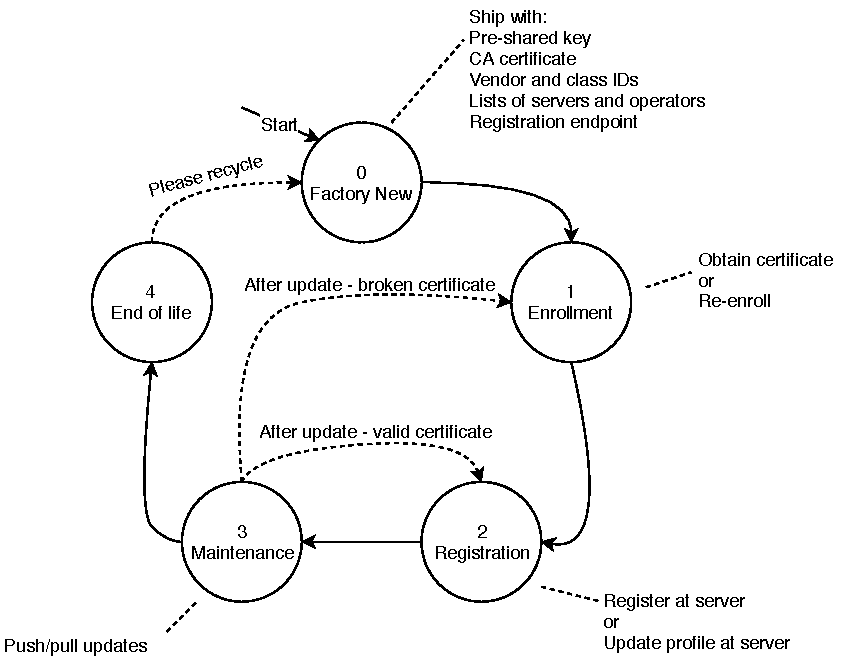
\includegraphics{images/lifecycle.pdf}
\end{figure}


As discussed, a factory new device that is to be installed in an IoT network needs some
information in order to enroll and register at a server. A pre-shared key, CA certificate,
vendor and class IDs, list of servers and operators, and and endpoint for registration is
needed. These parts make sure the device can take part of the network and move to the next
step of the life cycle. 

Entering the enrollment stage, devices obtain certificates by enrolling at the CA. For
this the pre-shared key and CA certificate is needed. After obtaining a certificate the
device can be trusted by the servers. It registers at its designated servers who all
create a profile for the device. The device is now ready to be updated, and proceeds to
the maintenance stage.

The maintenance state can be expected to last for several years, and this is where the
device receives and applies updates. As updates can change the capabilities of devices, by
for instance implementing a new transport protocol in software, devices should confirm
successful updates at the server so the server can build a new profile for that device.
Servers also need to be updated with the new version the device is running, which further
motivates the update confirmation. This means after an update, the device will either move
back to the enrollment or registration stage.

If certificates are broken after updates, as discussed in Section~\ref{sec:key-management},
devices move back to the enrollment stage to obtain a new certificate. If the certificate
is still valid after the update, the device moves back to the registration stage, updates
the profile at the servers, and then moves back to maintenance. The device will remain in
the maintenance stage until it either breaks or is taken out of service. If you are a
manufacturer of IoT devices please consider recycling or (securely) re-using devices,
starting the life cycle anew.


\section{Different Architectures}
\label{ssec:different-architectures}
As discussed, operators, servers, and devices can interact in many ways. The architecture
tries to be flexible allowing for different network topologies and configurations. The
important parts are that devices can enroll and register, all actors have valid
certificates, and that updates can be authorized. 

Figure~\ref{fig:operator-direct} shows an example architecture with one operator, one
server, and one device. The operator is capable of running the protocols needed to
communicate in the constrained network, and can thus interact directly with both the
device to send manifests and server to send images. An architecture like this allows for
servers to be distributed within the constrained network, possibly as more capable IoT
devices.

\begin{figure}
    \caption{An operator communicating directly with machines in the constrained network.}
    \label{fig:operator-direct}
    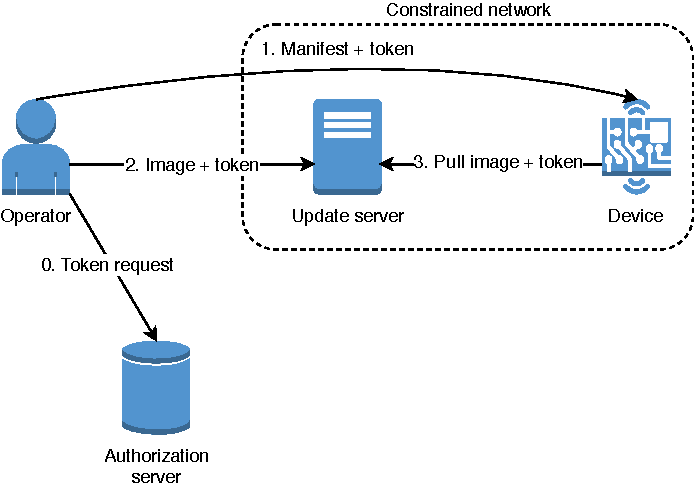
\includegraphics{images/operator-direct.pdf}
\end{figure}

Figure~\ref{fig:operator-proxy} shows an operator 

\begin{figure}
    \caption{}
    \label{fig:operator-proxy}
    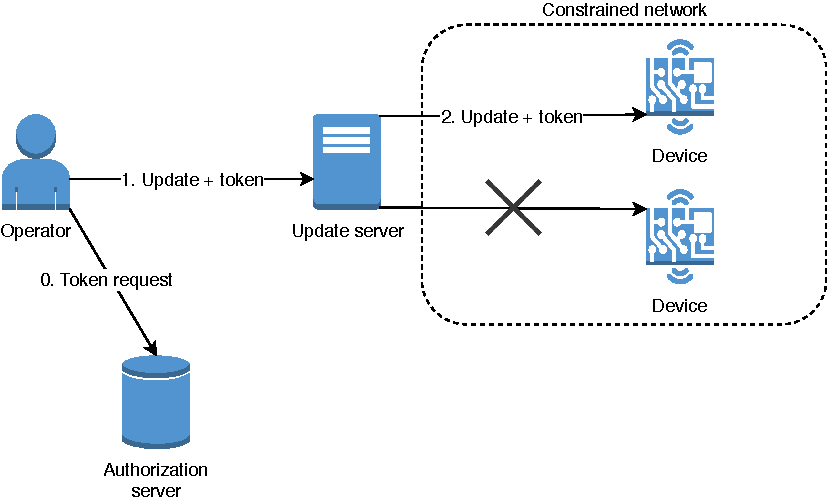
\includegraphics{images/operator-indirect.pdf}
\end{figure}

Figure~\ref{fig:operator-server} shows a third alternative 

\begin{figure}
    \caption{}
    \label{fig:operator-server}
    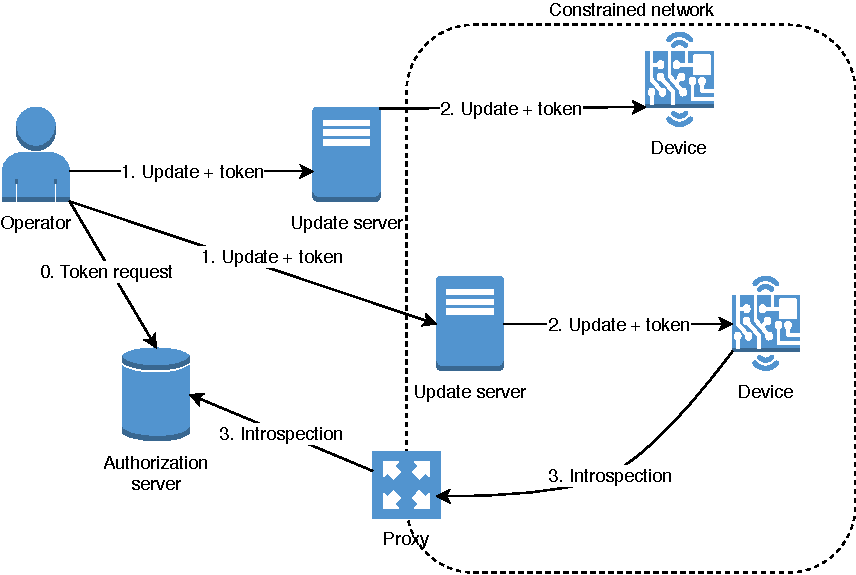
\includegraphics{images/operator-introspection.pdf}
\end{figure}

There are many other possible architectures and configurations. What these three examples
have in common is that the operator always resides outside the constrained network,
devices always reside within the constrained network, and that servers transport updates
to devices. In turn, devices register and update their statuses to the servers. Since
operators reside in traditional networks using traditional protocols such as HTTP over
TCP, a proxy mechanism may be necessary to communicate with the often UDP based
constrained networks. Remember from Section~\ref{ssec:coap} that CoAP can easily be
proxied to and from HTTP meaning a server running for instance CoAP could also be used as
a proxy for the operator. If the operator has the proper protocols implemented, they could
communicate manifests directly to a device.

\end{document}